%!TEX root = Bericht.tex
\graphicspath{{graphics/}}

\chapter{Trajectory Planning}
\label{cha:trajectory}
For the two most advanced modes, i. e. the Half-Automatic and the Full-Automatic Mode, trajectories had to be generated. In this chapter the best trajectories for \textsc{Skye} are elaborated and tested with suitable trajectory controllers. Performance results based on a \textsc{Matlab} simulation are shown.

%\subsection{Our Approach}
%From the GUI it was given that the goal trajectory would be a multipoint-interpolating %trajectory. The user is able to define waypoints on a map which afterwards should be %connected with a reasonable and realizable trajectory. Beside interpolating trajectories %there exist also approximating trajectories but they were not taken into consideration, since %usually the user wants skye fly directly through a waypoint.

%In another Bsc Thesis elaborated in this project a controller for waypoint following was %designed. So it was convenient in the scope of this Thesis to use this controller instead of %a specialized trajectory controller.

\section{Experimental Design}
The main application fields of the system \textsc{Skye} are image capturing and agile performance demonstrations. The waypoints used to test the trajectory algorithms had therefore to be alike these situations. All the results below belong to the three sample waypoints shown in figure \ref{fig:sampleNodes}. They represent standard situations for the applications mentioned before. Indeed, to verify the conclusions, some a wider set of waypoints had to be considered.
\\
The first waypoints are similar as they would be set to capture images of the the university building. 

\begin{figure}[h]
  \begin{minipage}[t]{0.32\textwidth}
    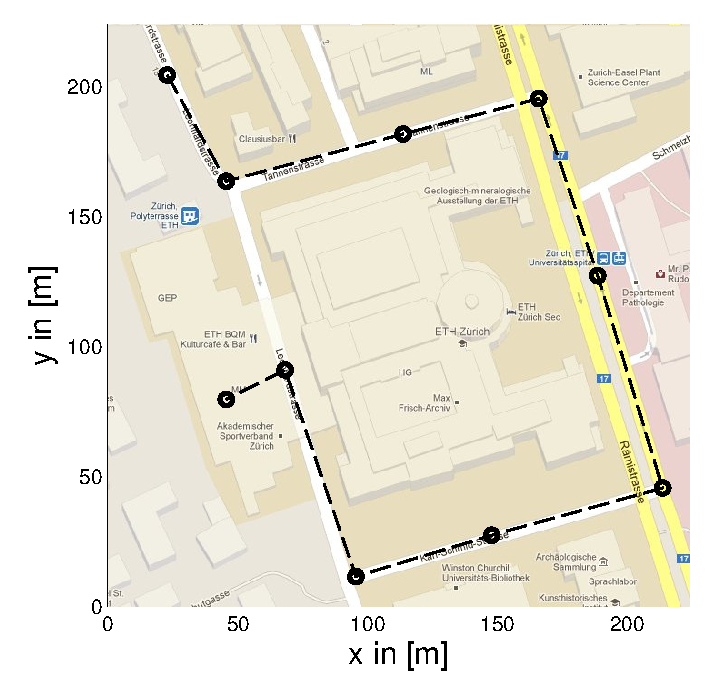
\includegraphics[width = \textwidth]{graphics/sampleNodeRoad}
  \end{minipage}
  \hfill
  \begin{minipage}[t]{0.32\textwidth}
    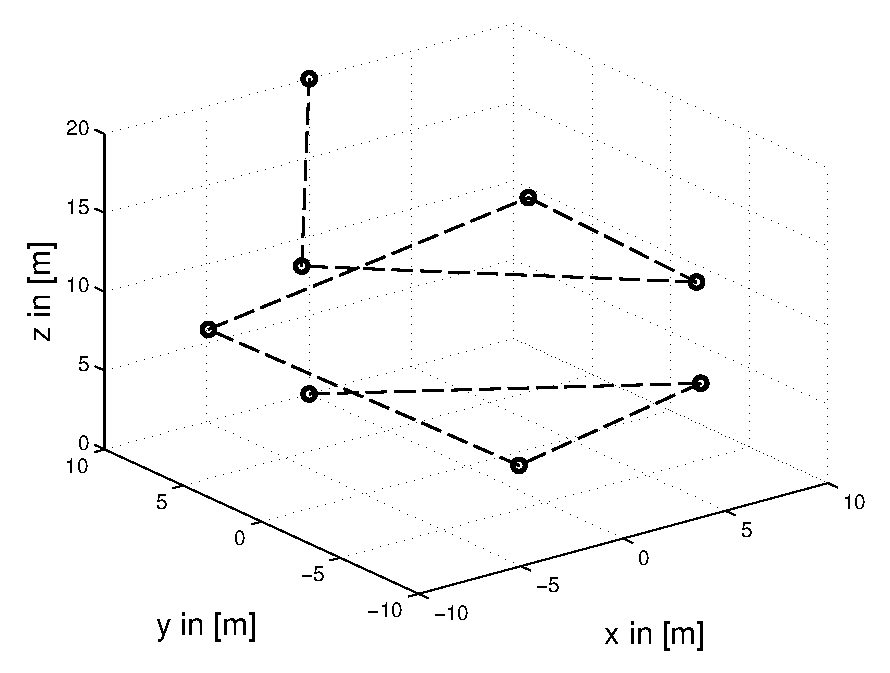
\includegraphics[width = \textwidth]{graphics/sampleNodeHelix}
  \end{minipage}
  \hfill
  \begin{minipage}[t]{0.32\textwidth}
    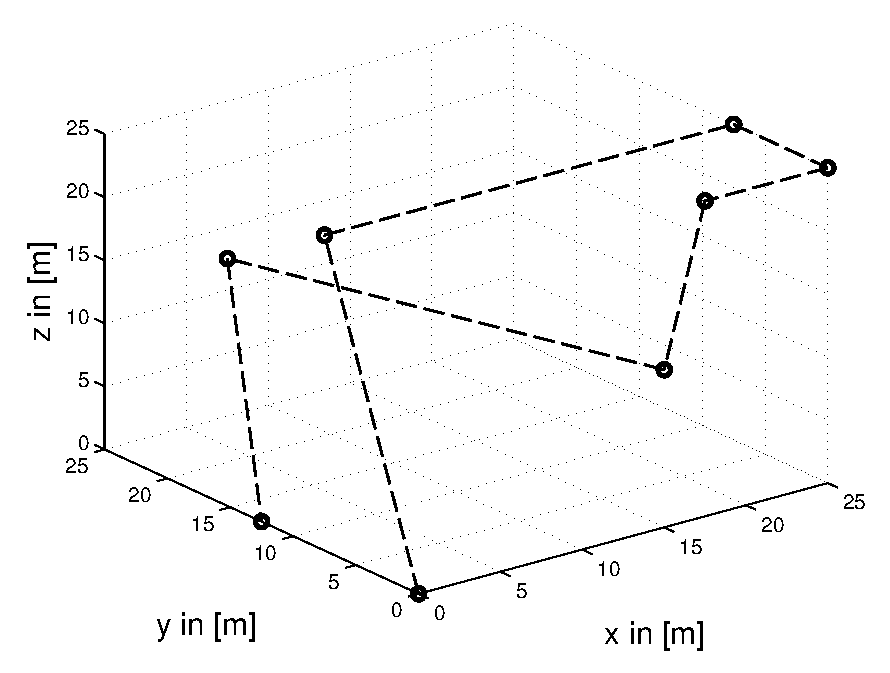
\includegraphics[width = \textwidth]{graphics/sampleNodeAgile}
  \end{minipage}
  \caption{The experimental environment based on three samples. {\bf Left:} The \textit{road} waypoints represent the need of low overshoots to not touch obstacles beside the streets. Its long straight ways enable high velocities. {\bf Center:} The \textit{helix} waypoints represents the circumnavigation of any obstacle. It yields to high curvatures of the track. {\bf Right:} The \textit{agile} waypoints include both straight sections as high curvatures.}
  \label{fig:sampleNodes}
\end{figure}


Furthermore, to score (\textbf{and optimize?}) the generated trajectories $\tilde{p}(t)$ and the resulting trace of the system $r(t)$, we set up the following criteria. Criteria (\ref{item:static_deviation}) to (\ref{item:static_acceleration}) are refered to as \textit{static criteria} as they do not depend any simulation. The remaining ones (\textit{dynamic criteria}) then mainly depend on the used controller\footnote{For detailed description of the used notation consider section \ref{sec:definition}}.
\\
Being $L_p$ the length of the path ${\bf p}(u)$ and $T_p$ the time of the trajectory $\tilde{\bf p}(t)$
\begin{equation}
L_p = \int_{u_{min}}^{u_{max}} du \qquad T_p = \int_{t_{min}}^{t_{max}} dt
\label{eq:length_of_path}
\end{equation}
the criteria are:

\begin{enumerate}[i)] 
\item Average deviation between actual path and chord connection between waypoints
\label{item:static_deviation}
\begin{equation}
J_1 = \int_{u_{min}}^{u_{max}} \|{\bf p}(u)- {\bf p}_2(u)\| du \cdot L_p^{-1} \label{eq:static_deviation}
\end{equation}

\item Average curvature of path\footnote{For a derivation of curvature see any vetor analysis book, e.g. \cite{stammbach} chapter II, page 71.}
\label{item:static_curvature}
\begin{equation}
J_2 = \int_{u_{min}}^{u_{max}} \frac{\| \frac{d {\bf p}}{du} \times \frac{d^{2} {\bf p}}{du^{2}} \|}{\|  \frac{d {\bf p}}{du} \|^3}du \cdot L_p^{-1}
\label{eq:static_curvature}
\end{equation}
% THIS ALTERNATIVE NOTATION IS INCONSEQUENCE IN USING DOT WHEN NOT HAVING PARAM T !!
% J_2 = \int_{u_{min}}^{u_{max}} \frac{\| \dot{\bf p}(u) \times \ddot{\bf p}(u) \|}{\| \dot{\bf p}(u) \|^3}du \cdot L_p^{-1}

\item Average acceleration of the trajectory
\label{item:static_acceleration}
\begin{equation}
J_3 = \int_{t_{min}}^{t_{max}} \|{\bf \ddot{\tilde{p}}}(t)\| dt \cdot T_p^{-1} \label{eq:static_acceleration}
\end{equation}

\item Deviation between trajectory and trace of the system\footnote{The deviation vector between trace and its closest point on the trajectory is always normal to the latter. Compare with figure \ref{fig:scene_crossTrack}.}
\label{item:dynamic_deviation}
\begin{equation}
J_4 = \int_{t_{min}}^{t_{max}} \| {\bf \tilde{p}}(t_{cl}) - {\bf r}(t) \| dt \cdot T_p^{-1} 
\label{eq:dynamic_deviation}
\end{equation}

\item Average acceleration of the system
\label{item:dynamic_acceleration}
\begin{equation}
J_5 = \int_{t_{min}}^{t_{max}} \|{\bf \ddot{r}}(t)\| dt \cdot T_p^{-1}
\end{equation}

\item Time synchronity\footnote{Time synchronity should be warranted for accurate \textit{trajectory} following. In our task for caputuring time independent imagery, it was only considered as a secondary aspect.}
\label{item:dynamic_synchronity}
\begin{equation}
J_6 = \| {\bf \tilde{p}}(t_{max}) - {\bf r}(t_{max}) \| \cdot L_p^{-1} \label{eq:dynamic_synchronity}
\end{equation}

\end{enumerate}


\section{Definition of Trajectories}
\label{sec:definition}
\subsection{Paths and Trajectories}
The main difference between a path $ {\bf p}(u)$ and a trajectory $ {\bf \tilde{p}}(t)$ is that only the latter includes time, i.e. considers the dynamics. A path is only defined as the way to go from point a to point b. Therefore it only has geometrical properties. In order to generate a trajectory, a time needs to be assigned to each point on the path. This is done with a function $u=u(t)$ that connects the parameter $u$ of the geometrical path with the time. The composition of the function\footnote{In  \cite{snider} named as the \textit{Motion Law}} $u=u(t)$ and the geometrical path ${\bf p}(u)$ finally forms the trajectory ${\bf \tilde{p}}(t)$. This concept is shown in figure \ref{fig:path_trajectory}.
\begin{figure}[h]
\centering
\def\svgwidth{0.9\textwidth}
\input{graphics/PathTrajectory.pdf_tex}
\caption{Composition of a path ${\bf p}(u)$ and the motion law $u(t)$ forming the trajectory ${\bf \tilde{p}}(t)$}
\label{fig:path_trajectory}
\end{figure}

In order to get the velocity and acceleration of the trajectory, the chain rule has to be applied to ${\bf \tilde{p}}(t)=({\bf p}\circ u)(t)$:

\begin{align}\label{vel_acc}
{\bf \dot{\tilde{p}}}(t) &= \frac{d {\bf p}}{du}\dot{u}(t) \\
{\bf \ddot{\tilde{p}}}(t) &= \frac{d {\bf p}}{du}\ddot{u}(t)+\frac{d^{2} {\bf p}}{du^{2}}\dot{u}^{2}(t)
\end{align}

%{\bf \ddot{\tilde{p}}}(t)





\subsection{Interpolation and Approximation}
If one wants to draw a path through a set of waypoints, there exists two ways to do this. First, the path can pass through all waypoints no matter how many bends it will have. Secondly, the path tries to best fit waypoint set, i.e. a function of a  certain order is adopted to best fit the waypoints. This can be done with different methods, e.g with least-squares. The first approach is called interpolation whereas the second approach is called approximation. Depending on the choice, different curves with different properties are formed (see figure \ref{fig:ApproxInterpol}).  


\begin{figure}[H]
  \begin{minipage}[t]{0.9\textwidth}
    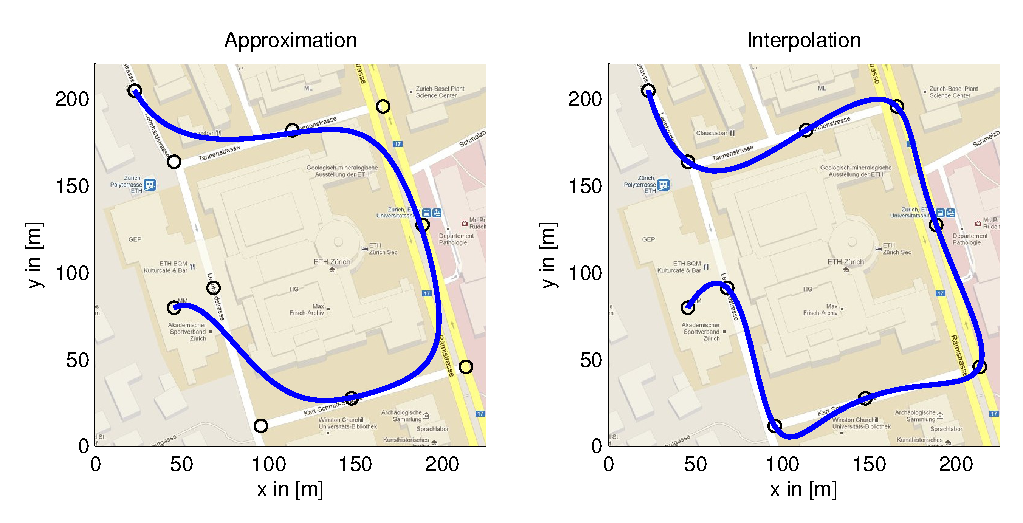
\includegraphics[width = \textwidth]{graphics/ApproxInterpol.eps}
  \end{minipage}
  \hfill
  \begin{minipage}[t]{0.8\textwidth}
%    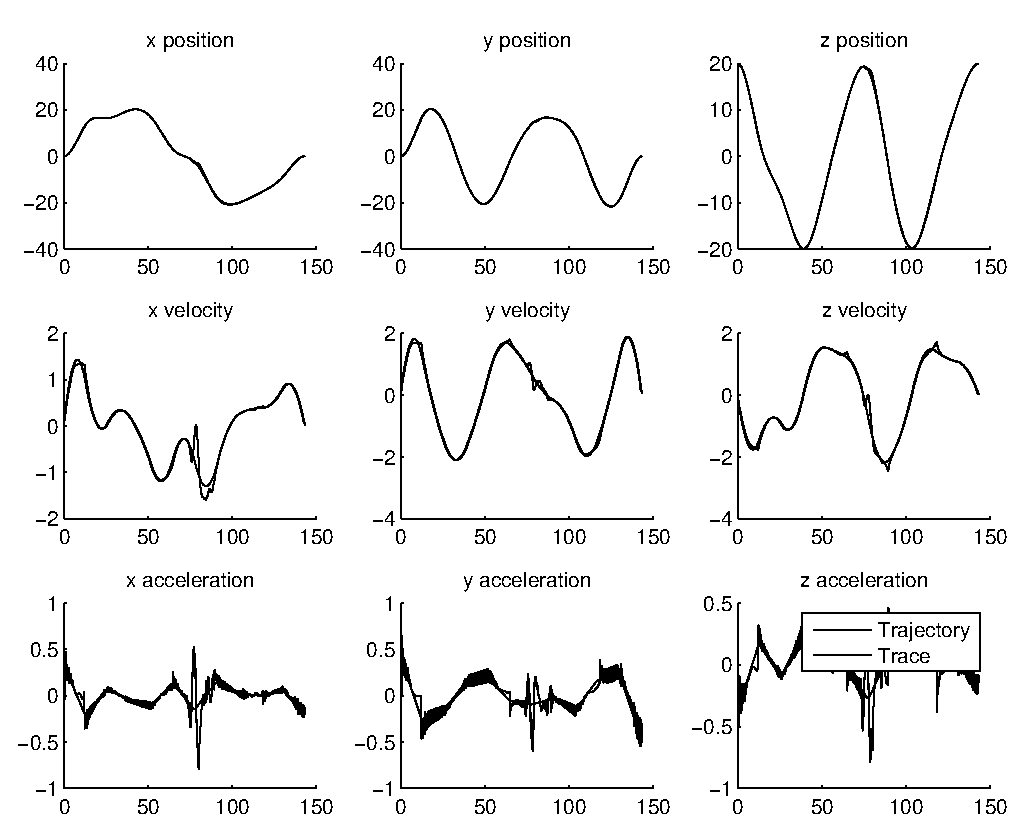
\includegraphics[width = \textwidth]{graphics/b.eps}
  \end{minipage}
  \caption{Interpolation and approximation of waypoints}
  \label{fig:ApproxInterpol}
\end{figure}

For the the trajectory planning for \textsc{Skye}, it was necessary to interpolate the waypoints. This was due to the GUI used (see \ref{sec:realization}). There only a small amount of waypoints is set ant the pilot expects the UAV to pass through all of them and not to take a shortcut. The approximation of the waypoints could result in a collision with buildings as shown in \ref{fig:ApproxInterpol}.


There mainly exist two solution to interpolate a given set of $n+1$ waypoints. A polynomial (of order $\ge n+1$) from $\varPi_{n}$ or else a set of polynomials of lower order, defined over a certain interval, can be used. This set of polynomials finally forms a spline. As impressively shown in \cite{wolfgang}, splines are the better option for more than a few waypoints. 

%A set of data points can be interpolated with one single curve or with a set of curves defined over a certain interval.  For a references to \cite{engeln}, \cite{biagiotti} and \cite{doessegger}


%\subsubsection{Continuity}
%\subsubsection{Boundary Conditions}
%\subsubsection{Polynomial Order}
%\subsubsection{Parametrization}
%\subsection{Piecewise Polynomial Interpolating Splines}
%\subsubsection{Boundary Conditions}
%\subsubsection{Polynomial Order}
%\subsubsection{Parameterization}
%\subsection{B-Splines}
%\subsubsection{Boundary Conditions}
%\subsubsection{Polynomial Order}
%\subsubsection{Parametrization}


\section{Splines}
\label{sec:splines}
\subsection{Parameterization}
Before actually a path can be drawn through a set of waypoints respectively a spline can be calculated, a value of the parameter $u$ needs to be assigned to all $n+1$ waypoints, i.e. a nondecreasing sequence of $u_0 < u_1 < ...< u_n$ must be found. In this section, the most common used techniques are analyzed\footnote{A vaster evaluation of different parameterization can be found in \cite{haron}} The choice of parameterization affects the geometrical properties of the path on the one hand and the velocity and acceleration of the trajectory on the other hand. (compare \eqref{vel_acc}). Latter is especially of big impact if a proportional relation is used to describe the motion law, i.e. $u=\lambda t$ (compare \ref{sec:motionLaw}).

\subsubsection{Uniform}
This is the simplest way to define the $u_{0-n}$. Here basically the index number of the waypoints are assigned to $u$. Therefore no meaningful interpretation can be made.
\begin{equation*}
u_n-u_{n-1}=1
\end{equation*}
\subsubsection{Chord length}
In this method the chord length between the waypoints is calculated and then summed up and assigned to $u$. With $u=\lambda t$ this method can be interpreted to aim for a more or less constant velocity over the whole trajectory.
\begin{equation*}
u_n-u_{n-1}=\left \| \begin{bmatrix}x_n\\y_n\\z_n \end{bmatrix}-\begin{bmatrix}x_{n-1}\\y_{n-1}\\z_{n-1} \end{bmatrix}\right \|
\end{equation*}
\subsubsection{Arc length}
The arc length method is improved version of the chord length distribution in order to reach a constant velocity. Here instead of taking the chord length between two waypoints, the arc length is estimated and summed up. The algorithm\footnote{The algorithm was taken from \cite{engeln} and implemented in \textsc{Matlab}.} for that can be found in \ref{sec:arcLengthDistribution}.
{\bf include picture}

\subsubsection{Centripetal}
This method was first proposed in \cite{lee}. Here the root of the chord length is used. The motivation for this method is that the larger the angular change from $\textnormal{waypoint}_{n-1}$ to $\textnormal{waypoint}_n$, the more centripetal force is accepted. A justification for this statement can be found in \cite{doessegger} and \cite{lee}.
\begin{equation*}
u_n-u_{n-1}=\sqrt{\left \| \begin{bmatrix}x_n\\y_n\\z_n \end{bmatrix}-\begin{bmatrix}x_{n-1}\\y_{n-1}\\z_{n-1} \end{bmatrix}\right \|}
\end{equation*}

\subsubsection{Comparison}
geometrical properties, dynamical properties, Kreb'sche Bewertungsalgrithmen:) \textbf{pictures of all of them, justify choice, say that if more waypoints, different decision}

\subsection{Spline Degree}
\subsubsection{Continuity}
first: explain, show continuity\\
second: Decision with Propulsion Dynamics and oscillation

\subsection{Boundary Conditions}

\subsection{implementation}


\section{Motion Law}
\label{sec:motionLaw}
\subsection{System Constraints}
\label{subsec:systemConstraints}
In order to plan a feasible trajectory one has to know the capabilities of the system. Here just a basic derivation for the velocities and accelerations is given, for more details refer to (!!!!Bsc Thesis Joe, Bsc Thesis Andy)\\

The maximum feasible acceleration in any direction is calculated to be:

\begin{equation}
  \left|a_{max} \right| =  \frac{\left|F_{res, w}\right|}{m_{tot}} = 0.96 m/s^2
\end{equation}

Whereas the $F_{res,w}$ is the force resulting from all four thrusters operated under full load in the worst direction and $m_{tot}$ is the sum of the masses of the helium, the virtual mass and the mass of the system itself.\\


The maximum feasible velocity in any direction is calculated to be:

\begin{equation}
\left|v_{max} \right| = \sqrt{\frac{\left|F_{res,w} \right|}{\frac{1}{2}c_d \rho \pi r^2}}=2.9 m/s
\end{equation}

which is nothing but $ \left|F_{res,min} \right| = \left|F_{dray} \right| $.\\

For trajectories for position and orientation the maximal feasible angular acceleration is also important. It is calculated to be:

\begin{equation}
  \left|\Psi_{max} \right| =  \frac{\left|M_{res,w}\right|}{\left| \lambda_{max, J_{B}} \right|} = 2.06 rad/s^2 
\end{equation}

which is quite conservative because it is assumed that worst axis for turning is also the principle axis of the inertia tensor with the highest inertia.\\

Since the system is almost undamped for rotations, the rotational velocities will never be the limiting factor.

\subsection{Time Scaling}
\label{timeScaling}

\section{Controller Implementation}
Some commonly used trajectory controllers\footnote{\cite{snider} provides a good overview to trajectory control.} are tested to follow the defined trajectories. The \textit{Trajectory following} controller supplies the system's position controller \cite{meier} with a feed forward reference signal. Although it delivers good results for ideal case, the tracking get worse for the non perfect model case. The \textit{pure pursuit} controller, which is based on a lookahead point as well as the \textit{cross track error} controller dynamically react on model uncertainties and yield therefore to more robust path tracking results.
\\
BLA BLA introduce notation.. $r(t)$ bla.

 XXXX see \cite{snider} and \cite{deluca}
\label{sec:controllerImplementation}
\subsection{Trajectory Following}
Assuming a perfect model and a trajectory considering all system constraints\footnote{I.e. saturations of $\dot{r}(t)$ and its derivatives.}, the position $r\left(t\right)$ of the system can be assumed to be equal to the trajectory $\tilde{p}(t)$ at any time. Therefore, a straight forward way of a trajectory controller is to follow the trajectory $\tilde{p}(t)$ for every time $t$. This yields to accurate tracking in a safe environment \cite{doesegger}.
\\
A position controller with feedforward terms for velocity and acceleration as described in \cite{meiermueri} can therefore be used with the reference input

\begin{equation}
  [r_{ref}(t), \; \dot{r}_{ref}(t), \; \ddot{r}_{ref}(t)]^T = [\tilde{p}(t), \; \dot{\tilde{p}}(t), \; \ddot{\tilde{p}}(t)]^T
\end{equation}

The controller scheme is shown in figure \ref{fig:trajectoryfollowing}. 

%$\left[ \begin{array}{c} {\bf r}(t) \\ {\bf \dot{r}}(t) \end{array} \right]$
\begin{figure}[h]
    \centering
    \def\svgwidth{0.4\columnwidth}
    \input{graphics/scene_trajectoryFollowing.pdf_tex}
    \caption{For a perfect model and a trajectory ${\bf \tilde{p}}(t)$ considering all system constraints, the position ${\bf{r}}(t)$ will correctly follow the trajectory.}
    \label{fig:scene_trajectoryFollowing}
\end{figure}

\begin{figure}[h]
    \centering
    \def\svgwidth{\columnwidth}
    \input{graphics/controller_trajectoryFollowing.pdf_tex}
    \caption{Trajectory following controller. The value of the parameter $t$ of the trajectory is equal to the current time.}
    \label{fig:trajectoryfollowing}
\end{figure}


Testing the controller yields good performance.. BLA BLA Graphic figure 



\subsection{Pure Pursuit Controller}
Another commonly used trajectory controller is Pure Pursuit \cite{snider}. To consider all dynamics of the trajectory, the reference intput is based on a lookahead point $\tilde{p}(t_{cl}+\Delta T) = {\bf \tilde{p}}(t_{cl}) + \Delta T \cdot {\bf\dot{ \tilde{p}}}(t_{cl}) + \frac{1}{2} \Delta T^2 \cdot {\bf\ddot{ \tilde{p}}}(t_{cl}) + \mathcal{O}(\Delta T^3)$ that considers terms of ${\bf \tilde{p}}(t)$ and all its derivatives\footnote{Note, that this is a simple and robust alternative to any derivative controller.}.

%$ {\bf \dot{r}}_{ref}(t) $
\begin{figure}[h]
    \centering
    \def\svgwidth{0.5\columnwidth}
    \input{graphics/scene_purePursuit.pdf_tex}
    \caption{Pure pursuit yields to extremly awesome tracking.}
    \label{fig:scene_purePursuit}
\end{figure}

\begin{figure}[h]
    \centering
    \def\svgwidth{\columnwidth}
    \input{graphics/controller_purePursuit.pdf_tex}
    \caption{Pure pursuit yields to extremly awesome tracking.}
    \label{fig:purePursuit}
\end{figure}

\subsection{Cross Track Error Controller}
see \cite{williams}

%$\left[ \begin{array}{c} {\bf \tilde{p}}(t) \\ {\bf \dot{\tilde{p}}}(t) \\ {\bf \ddot{\tilde{p}}}(t) \end{array} \right]$
\begin{figure}[h]
    \centering
    \def\svgwidth{0.5\columnwidth}
    \input{graphics/scene_crossTrack.pdf_tex}
    \caption{Cross Track Error Control yields to extremly awesome tracking.}
    \label{fig:scene_crossTrack}
\end{figure}


\begin{figure}[h]
    \centering
    \def\svgwidth{\columnwidth}
    \input{graphics/controller_crossTrack.pdf_tex}
    \caption{Cross Track Error Control yields to extremly awesome tracking.}
    \label{fig:crossTrack}
\end{figure}

\section{Discussion}
\label{sec:discussion}

